\section{Dense predictive features and world action coupling in 2026}
\label{sec:C05:frontier}
V-JEPA 2.1 changes the training target rather than merely scaling the original video encoder. Its Section 2.3 applies prediction supervision to masked and visible tokens, introduces intermediate-layer supervision, and uses modality-specific image/video patch embeddings. The inspected 2026 implementation exposes \path{forward_target}, \path{forward_context}, and \path{loss_fn} in \path{app/vjepa_2_1/train.py}~\cite{rewrite_vjepa21,rewrite_vjepa2_repo}. This is a current, identifiable objective-to-code case; the original I-JEPA discussion supplies its foundation rather than a claim about the frontier's latest recipe.

The local-versus-global tradeoff has a useful optimization interpretation. Let $L_m$ measure prediction of masked targets and $L_c$ supervision of visible context features. Training minimizes $L_m+\lambda L_c$ in a simplified two-term view. A direction that reduces $L_c$ can increase $L_m$ when the gradient inner product is negative. Thus adding dense supervision is not guaranteed to improve every global metric. The scale and spatial weighting of the context term determine which distinctions receive pressure. This deduction explains why an implementation must retain the actual loss weights and scheduling, rather than treating the presence of an additional loss as a uniformly beneficial feature.

For agents, dense features are attractive because many operations depend on a localized affordance rather than a whole-scene label. The corresponding falsifiable hypothesis is that improved local representations reduce target-selection errors under a fixed policy and observation budget. Test that hypothesis with counterfactual layouts, small text, occlusion, and temporal changes. Retain a global-recognition diagnostic to detect whether the local gain trades away broader scene understanding. A classifier or robotics score from the source paper does not answer the computer-use question automatically; it identifies a mechanism worth testing.

Implementation inspection should follow the feature path across encoder layers, normalization, fusion, and predictor outputs. Multi-level features increase the amount of intermediate state that may be retained or recomputed. A frozen feature-extraction benchmark should include preprocessing and feature-transfer costs, not only encoder FLOPs. An agent that invokes the encoder on every observation may prefer a smaller distilled model, a crop policy, or event-triggered refresh even when a larger model has the best unconstrained representation score. Quality should therefore be plotted against complete decision latency and storage, with the action interface held constant.

The October 2026 revision of V-JEPA Policy couples a frozen V-JEPA 2.1 encoder with an instruction-conditioned future-latent predictor and a flow-matching action expert. Its Section 3 connects future-informed context keys and values to action generation, while the experiments compare visual foundations under a common downstream framework~\cite{rewrite_vjepapolicy2026}. This is a more direct representation-to-action case than passive recognition alone. It still changes several trained components, so a result for the complete policy cannot be assigned entirely to the frozen encoder without the corresponding controlled comparison.

The actual coupling point matters for an ablation. The action expert reads the predictor's layerwise context keys and values, not the final future-latent readouts. In the paper's notation, its visual interface is
\begin{equation}
 \mathcal C_\phi=
 \{(\mathcal R_{\mathrm{3D}}(K_c^{(j)}),V_c^{(j)})\}_{j=1}^{L},
\end{equation}
where $K_c^{(j)},V_c^{(j)}$ are projections at context positions and only the keys receive the stated rotary transform~\cite{rewrite_vjepapolicy2026}. Changing an unused final readout would therefore not test whether the action path uses future-conditioned context. A more diagnostic proposed study holds the visual encoder and action expert fixed and intervenes on future-query-to-context interactions, preserving observed tokens, positions, tensor shapes and comparable compute. A performance drop after that intervention can support functional use of the coupling, while leaving its calibration and interventional validity open. Shuffling the whole context interface would conflate loss of present evidence with loss of future conditioning. Out-of-distribution corruption remains an alternative explanation and requires matched controls; no such experiment is reported here.



% SCIENTIFIC_FIGURE_C05
Figure~\ref{fig:C05:overview} separates latent prediction from the downstream control path whose validity must be tested.
\begin{figure}[!htbp]
\centering
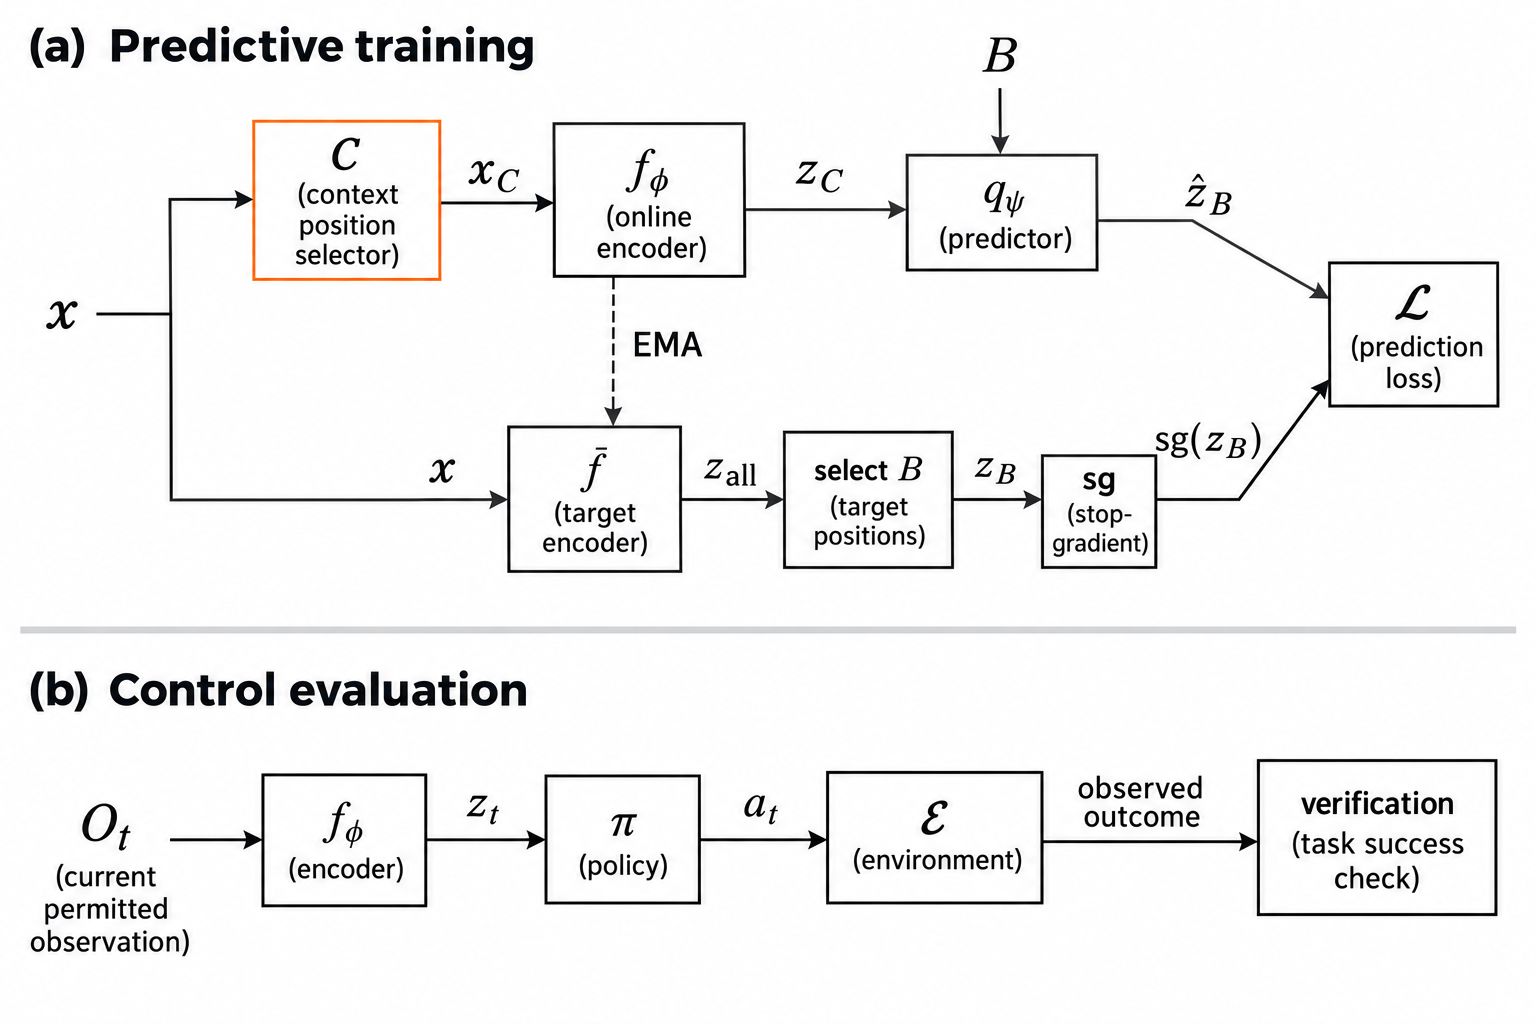
\includegraphics[width=\linewidth]{book/figures/assets/F05review.png}
\caption{Predictive representation training and control test different properties. The context branch uses positions $C$; the target branch processes the complete observation, selects positions $B$, and blocks loss gradients through $\mathrm{sg}$. An EMA parameter update is separate from gradient flow. The declared loss must match the selected JEPA variant. A downstream controller requires independent environment-outcome evaluation; small prediction loss does not establish action sufficiency.}
\label{fig:C05:overview}
\end{figure}
